\section{Resultats}
\label{sec:resultats}

\subsection{resultats première expérience}

Les resultats de la première expérience sont montrés dans la \figref{renaming}. Tout d'abord, le nombre de renommage varie beaucoup entre les projets. Par exemple Jenkins a au plus $10\%$ de ses fichiers renommés dans la pire période alors que PHPUnit a deux périodes à plus de $50\%$. Le nombre de renommages varie aussi en fonction des périodes, par exemple dans PHPUnit la période $3.6 - 3.7$ a moins de $5\%$ de fichiers renommés alors que la période $3.7 - 4.0$ a presque $99\%$. En général, il y a beaucoup de périodes avec $0\%$ de fichiers renommés\\

Par rapport à la localisation de ces renommages, la période initial semble la pire. En général elle contient le plus grand nombre de fichiers renommés (sauf pour PHPUnit). Les périodes de développement sont plus susceptible d'avoir des renommages que les périodes de maintenances, tels que les $5$ projets sont quasiment à $0\%$ de fichiers renommés dans les périodes de maintenance (voir tableaux détails). Finallement, certaines périodes de développement peuvent contenir beaucoup de renommages. Les résultats montrent que les releases majeurs sont souvent les pires périodes de développement en nombre de fichiers renommés: C'est le cas pour PHPUnit et Rails alors que Jenkins et Pyramid ne contiennent pas de releases majeur.\\ 

\begin{figure*}[t]
	\centering
	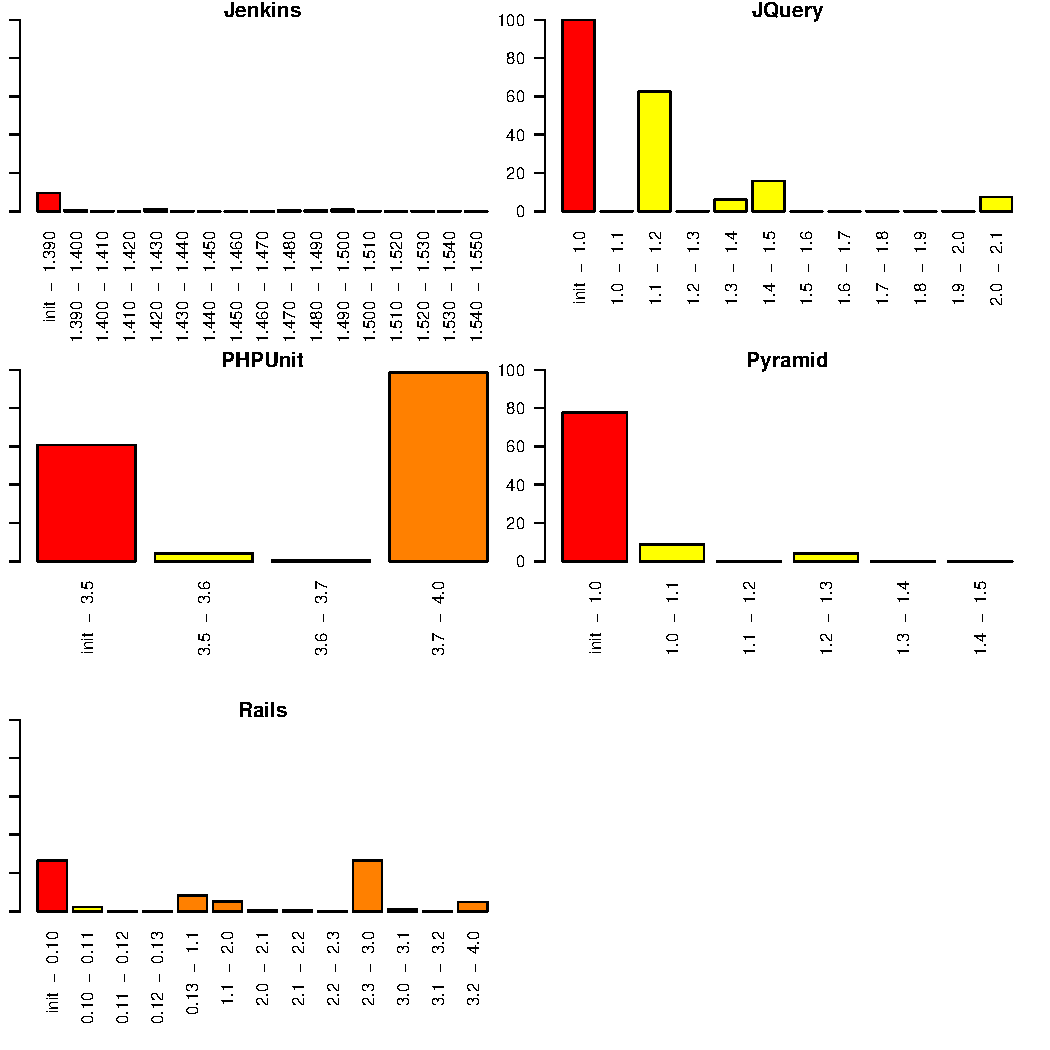
\includegraphics[width=0.85\linewidth,keepaspectratio]{data/figures/renaming.pdf}
	\caption{Percentage of files renamed ($\%F_R$) in each period of each project of our corpus. The initial period is in dark grey, major periods are in medium grey and minor periods are in light grey.}
	\label{fig:renaming}
\end{figure*}


Le détail des résultats obtenus par notre outil de détection de renommage sont montrés dans les tables \tabref{jenkins}, \tabref{jquery}, \tabref{phpunit}, \tabref{pyramid} et \tabref{rails}.\\

\begin{itemize}
\item \emph{Number of files ($\#F$):} number of files in the project at the last version of the period.
\item \emph{Number of active files ($\#AF$):} number of files created, deleted, copied, modified or renamed during the period and present at the last version of the period.
\item \emph{Percentage of active files ($\%AF$):} $\%AF = \frac{\#AF}{\#F}$.
\item \emph{Number of renamed active files ($\#AF_{r}$):} number of active files that have been renamed.
\item \emph{Percentage of files renamed ($\%F_{R}$):} $\%F_{R} = \frac{\#AF_{R}}{\#F}$.
\item \emph{Percentage of active files renamed ($\%AF_{R}$):} $\%AF_{R} = \frac{\#AF_{R}}{\#AF}$.
\end{itemize}

\begin{table}
\centering
\scriptsize
\csvreader[tabular=rcccccc, table head=\toprule & & \multicolumn{5}{c}{Renaming metrics}\\\cmidrule{3-7} Period & Kind & $\#F$ & $\#AF$ & $\%AF$ & $\%F_r$ & $\%AF_r$\\\midrule, late after line=\\, late after last line=\\\bottomrule, after table=]{data/tables/jenkins.csv}%
{1=\period,2=\kind,3=\nf,4=\naf,5=\paf,6=\pfr,7=\pafr}%
{\period & \kind & \nf & \naf & \paf & \pfr & \pafr}
\caption{Amount and location of renaming in Jenkins}
\label{tab:jenkins}
\end{table}

\begin{table}
\centering
\scriptsize
\csvreader[tabular=rcccccc, table head=\toprule & & \multicolumn{5}{c}{Renaming metrics}\\\cmidrule{3-7} Period & Kind & $\#F$ & $\#AF$ & $\%AF$ & $\%F_r$ & $\%AF_r$\\\midrule, late after line=\\, late after last line=\\\bottomrule]{data/tables/jquery.csv}%
{1=\period,2=\kind,3=\nf,4=\naf,5=\paf,6=\pfr,7=\pafr}%
{\period & \kind & \nf & \naf & \paf & \pfr & \pafr}
\caption{Amount and location of renaming in JQuery}
\label{tab:jquery}
\end{table}

\begin{table}
\centering
\scriptsize
\csvreader[tabular=rcccccc, table head=\toprule & & \multicolumn{5}{c}{Renaming metrics}\\\cmidrule{3-7} Period & Kind & $\#F$ & $\#AF$ & $\%AF$ & $\%F_r$ & $\%AF_r$\\\midrule, late after line=\\, late after last line=\\\bottomrule]{data/tables/phpunit.csv}%
{1=\period,2=\kind,3=\nf,4=\naf,5=\paf,6=\pfr,7=\pafr}%
{\period & \kind & \nf & \naf & \paf & \pfr & \pafr}
\caption{Amount and location of renaming in PHPUnit}
\label{tab:phpunit}
\end{table}

\begin{table}
\centering
\scriptsize
\csvreader[tabular=rcccccc, table head=\toprule & & \multicolumn{5}{c}{Renaming metrics}\\\cmidrule{3-7} Period & Kind & $\#F$ & $\#AF$ & $\%AF$ & $\%F_r$ & $\%AF_r$\\\midrule, late after line=\\, late after last line=\\\bottomrule]{data/tables/pyramid.csv}%
{1=\period,2=\kind,3=\nf,4=\naf,5=\paf,6=\pfr,7=\pafr}%
{\period & \kind & \nf & \naf & \paf & \pfr & \pafr}
\caption{Amount and location of renaming in Pyramid}
\label{tab:pyramid}
\end{table}

\begin{table}
\centering
\scriptsize
\csvreader[tabular=rcccccc, table head=\toprule & & \multicolumn{5}{c}{Renaming metrics}\\\cmidrule{3-7} Period & Kind & $\#F$ & $\#AF$ & $\%AF$ & $\%F_r$ & $\%AF_r$\\\midrule, late after line=\\, late after last line=\\\bottomrule]{data/tables/rails.csv}%
{1=\period,2=\kind,3=\nf,4=\naf,5=\paf,6=\pfr,7=\pafr}%
{\period & \kind & \nf & \naf & \paf & \pfr & \pafr}
\caption{Amount and location of renaming in Rails}
\label{tab:rails}
\end{table}

\subsection{resultats deuxième expérience}
Les résultats de notre deuxième expérience sont montrés dans la \tabref{spearman}. Ils montrent que la corrélation de coéficiants de Spearman entre les métriques de procédés avec et sans détection de renommages dépendent beaucoup de la période et de la métrique choisi. Les métriques de procédés ne sont pas affectés par le renommage dans les projets Jenkins, Rails et Pyramid tels que le coéficiant de corrélation est proche de $1$ dans tout les cas. D'un autre côté, pour PHPUnit et JQuery les métriques peuvent être sévèrement impactés par le renommage. Pour JQuery, la métrique Code Churn n'est pas affectée par le renommage, mais NoD et NoC sont quant à eux significativement impactés. Pour PHPUnit, toute les métriques sont affectés par le renommage. Sur ces deux derniers projets, la métriques la plus sensible au renommages de fichiers est le nombre de développeurs (NoD). Dans ce cas, nos résultats pourraient sérieusement invalider une étude effectué  sur ces périodes en utilisant ces métriques.\\
Finallement on peut noter que seules les périodes ayant eu un grand pourcentage de fichiers renommés ($\%F_R$) ont étés impactés. On peut aussi noter que des métriques biaisés par le renommage ont été calculés dans des releases majeur et mineur.\\

Nous avons étudiés manuellement les deux périodes qui ont affectés les valurs des métriques de procédés (JQuery 1.1 - 1.2 et PHPUnit 3.7 - 4.0). Nous avons remarqués que dans ces deux périodes, les structures principales des projets avaient étés significativement modifiés avec des renommages de dossiers de base. Par conséquent un grand nombre de fichiers ont étés renommés de manière transitive. C'est une pratique courante dans le développement logiciel, donc le phénomène pourrait apparaitre dans n'importe quel période ou projet. Il est intéressent de noter que dans ces deux périodes les changements de structure ont été effectués en grande partie dans un seul commit proche de la fin de la période.\\

\begin{table*}[t]
\centering
\small
\csvreader[tabular=rcccc, table head=\toprule & & \multicolumn{3}{c}{Change metrics}\\\cmidrule{3-5} Period & $\%F_R$ & CC & NoD & NoC\\\midrule, late after line=\\, late after last line=\\\bottomrule]{data/tables/correlations.csv}%
{1=\period,2=\fr,3=\churnall,4=\devall,5=\modificationsall}%
{\period & \fr & \churnall & \devall & \modificationsall}
\caption{Spearman correlation coefficients between values of change metrics with and without renaming. The significance codes are: *** $\leq 0.01$, ** $\leq 0.05$, * $\leq 0.1$ and ! $> 0.1$. Medium and low correlation coefficients are displayed in bold.}
\label{tab:spearman}
\end{table*}


\subsection{vérifications}
